\addtocontents{toc}{\protect\vfill\newpage}  %ToC would split algorithms chapter otherwise
\chapter{Algorithms} \label{chap:algorithms}

The iterations and data accessors described in the previous Chapters allow for a plethora of algorithms.
Most of them make use of basic functionalities such as the inner product of vectors, or the volume of a $n$-cell.
{\ViennaGrid} ships with a number of such basic tools, which are listed in Tab.~\ref{tab:algorithms} and discussed in the following.

The individual algorithms are located in the \lstinline|viennagrid/algorithm/| folder.
A tutorial covering the algorithms explained in this chapter can be found in \lstinline|examples/tutorial/algorithms.cpp|.


\TIP{Make sure to include the respective header-file when using one of the algorithms explained below!}

\begin{table}
 \begin{tabular}{|l|l|l|}
  \hline
   Algorithm & Filename   & Interface Function\\
   \hline
   Angles            & \texttt{angle.hpp}           & \lstinline|angle(origin, p0, p1)| \\
   Cross Product     & \texttt{cross\_prod.hpp}     & \lstinline|cross_prod(a, b)| \\
   Determinant       & \texttt{geometry.hpp}        & \lstinline|determinant(a, b, ...)| \\
   Induced Volume    & \texttt{spanned\_volume.hpp} & \lstinline|spanned_volume(a, b, ...)| \\
   Inner Product     & \texttt{inner\_prod.hpp}     & \lstinline|inner_prod(a, b)|\\
   Orthogonalization & \texttt{geometry.hpp}        & \lstinline|orthogonalize(p_begin, p_end, a)| \\
   Vector Norms      & \texttt{norm.hpp}            & \lstinline|norm(a, tag)| \\
   \hline
   Centroid computation & \texttt{centroid.hpp}           & \lstinline|centroid(element)| \\
   Circumcenter comp.   & \texttt{circumcenter.hpp}       & \lstinline|circumcenter(element)| \\
   Distance             & \texttt{distance.hpp}           & \lstinline|distance(element1, element2)| \\
   Normal vector        & \texttt{geometry.hpp}           & \lstinline|normal_vector(element)| \\
   %Quantity transfer    & \texttt{quantity\_transfer.hpp} & \lstinline|quantity_transfer(...)|\\
   Surface computation  & \texttt{surface.hpp}            & \lstinline|surface(element)| \\
   Volume computation   & \texttt{volume.hpp}             & \lstinline|volume(element)| \\
   \hline
   Affine transformation & \texttt{geometric\_transform.hpp}  & \lstinline|affine_transform(mesh, matrix, p)| \\
   Boundary detection    & \texttt{boundary.hpp}              & \lstinline|is_boundary(domseg, element)|\\
   Bounding box          & \texttt{geometry.hpp}              & \lstinline|bounding_box(mesh)|\\
   Closest points        & \texttt{closest\_points.hpp}       & \lstinline|closest_points(element1, element2)| \\
   Distance              & \texttt{distance.hpp}              & \lstinline|distance(element1, element2)| \\
   Extract boundary      & \texttt{extract\_boundary.hpp}     & \lstinline|extract_boundary(mesh_in, mesh_out)| \\
   Extract seed points   & \texttt{extract\_seed\_points.hpp} & \lstinline|extract_seed_points(mesh, cont)| \\
   Hyperplane refinement & \texttt{hyperplane\_refine.hpp}    & \lstinline|hyperplane_refine(...)| \\
   Interface detection   & \texttt{interface.hpp}             & \lstinline|is_interface(seg1, seg2, element)|\\
   Mesh size             & \texttt{geometry.hpp}              & \lstinline|mesh_size(mesh)|\\
   Quantity transfer     & \texttt{quantity\_transfer.hpp}    & \lstinline|quantity_transfer(...)|\\
   Simplex refinement    & \texttt{refine.hpp}                & \lstinline|refine(tag, mesh)| \\
   Scale mesh            & \texttt{geometric\_transform.hpp}  & \lstinline|scale(mesh, factor, center)| \\
   Surface computation   & \texttt{surface.hpp}               & \lstinline|surface(meshseg)| \\
   Volume computation    & \texttt{volume.hpp}                & \lstinline|volume(meshseg)| \\
   Voronoi grid          & \texttt{voronoi.hpp}               & \lstinline|apply_voronoi(meshseg, ...)| \\
   \hline
 \end{tabular}
 \caption{List of algorithms available in \texttt{viennagrid/algorithm/} grouped by the objects they are acting on. Additional overloads may be available.
    \lstinline|a| and \lstinline|b| denote vectors, \lstinline|p_begin| and \lstinline|p_end| refer to begin- and end-iterators over vectors, \lstinline|element| to an element,
    \lstinline|mesh| to a mesh, \lstinline|seg1| and \lstinline|seg2| to segments, and \lstinline|meshseg| to either a mesh or a segment.}
 \label{tab:algorithms}
\end{table}


\section{Point/Vector-Based}
This section details algorithms in {\ViennaGrid} requiring geometric information only.
The point type in {\ViennaGrid} should be seen in this context mostly as a vector type rather than a representation of a geometric location, reflecting the duality of points and vectors in the Euclidean space.

  \subsection{Angles}
 To compute the angle between two vectors pointing from the origin to points \lstinline|p1| and \lstinline|p2|, call
 \begin{lstlisting}
  viennagrid::angle(p1, p2);
 \end{lstlisting}
 If the vectors should have another common point \lstinline|p3| which acts as a translated origin, use
 \begin{lstlisting}
  viennagrid::angle(p1, p2, p3);
 \end{lstlisting}
 which is equivalent to calling
 \begin{lstlisting}
  viennagrid::angle(p1-p3, p2-p3);
 \end{lstlisting}

 In a three-dimensional coordinate system one can in addition compute the solid angle defined by three points with respect to the origin via
 \begin{lstlisting}
  viennagrid::solid_angle(p1, p2, p3);
 \end{lstlisting}
 If the solid angle should be determined with respect to another point \lstinline|p4|, use
 \begin{lstlisting}
  viennagrid::solid_angle(p1, p2, p3, p4);
 \end{lstlisting}

 The dihedral angle of two planes given by the points (\lstinline|a1|, \lstinline|a2|, \lstinline|a3|) and (\lstinline|b1|, \lstinline|b2|, \lstinline|b3|), respectively, is computed using
 \begin{lstlisting}
  viennagrid::dihedral_angle(a1, a2, a3, b1, b2, b3);
 \end{lstlisting}

  \subsection{Cross Products}
 The cross-product of two vectors (i.e.~{\ViennaGrid} points) \lstinline|p0| and \lstinline|p1| is defined for the three-dimensional space and computed with {\ViennaGrid} as
 \begin{lstlisting}
  viennagrid::cross_prod(p0, p1)
 \end{lstlisting}
 The following code calculates and prints the cross-product of the vectors $(1,0,0)^\mathrm{T}$ and $(0,1,0)^\mathrm{T}$:
 \begin{lstlisting}
  PointType p0(1, 0, 0);
  PointType p1(0, 1, 0);
  std::cout << viennagrid::cross_prod(p0, p1) << std::endl; //0 0 1
 \end{lstlisting}
 If the two vectors are given in different coordinate systems, the result vector will have the same coordinate system as the first argument.

 \subsection{Determinant}
 The determinant of the matrix obtained from writing $n$ vectors (points) of dimension $n$ into a square $n\times n$-matrix is a basic building block for several algorithms.
 Rather than extracting the coordinates of individual points, the determinant can be directly computed by passing the respective points to \lstinline|viennagrid::determinant()|:
 \begin{lstlisting}
  PointType p0(1, 0, 0);
  PointType p1(0, 1, 0);
  PointType p2(0, 0, 1);
  std::cout << viennagrid::determinant(p0, p1, p2) << std::endl;  //1
 \end{lstlisting}
 and similarly for the two-dimensional as well as the one-dimensional case.

 \subsection{Induced Volume}
 The volume of $n+1$ vectors spanning a simplex (line, triangle, tetrahedron...) in the $n$-dimensional space is computed via e.g.
 \begin{lstlisting}
  PointType p0(0, 0);
  PointType p1(0, 1);
  PointType p2(1, 0);
  std::cout << viennagrid::spanned_volume(p0, p1, p2) << std::endl;  //0.5
 \end{lstlisting}
 for the two-dimensional case. If the signed volume taking the orientation of vectors into account is required, use \lstinline|signed_spanned_volume()|.

  \subsection{Inner Products}
 Unlike cross products, inner products (aka.~dot products) are well defined for arbitrary dimensions. In {\ViennaGridversion} an inner product of the form
\begin{align}
 (\vector x, \vector y) = \sum_{i=0}^{N-1} x_i y_i
\end{align}
is available with the function \lstinline|inner_prod()|. The following code calculates and prints the inner product of the vectors $(1,0,0)^\mathrm{T}$ and $(0,1,0)^\mathrm{T}$:
 \begin{lstlisting}
  PointType p0(1, 0, 0);
  PointType p1(0, 1, 0);
  std::cout << viennagrid::inner_prod(p1, p2) << std::endl;  //0
 \end{lstlisting}
 If the two vectors are given in different coordinate systems, the result vector will have the same coordinate system as the first argument.

   \subsection{Orthogonalization}
 There are two different variants of orthogonalization implemented: The first orthogonalizes a single vector with respect to a container of given vectors:
 \begin{lstlisting}
  std::vector<PointType> basis;
  basis.push_back(PointType(1.0, 0.0, 0.0));
  basis_push_back(PointType(0.0, 1.0, 0.0));
  PointType p(1.0, 2.0, 3.0);
  std::cout << viennagrid::orthogonalize_vector(basis.begin(), basis.end(), p) << std::endl;  //0 0 3
 \end{lstlisting}
 The second version takes the set of vectors provided by the iterators and orthogonalizes all vectors using the Gram-Schmidt method:
 \begin{lstlisting}
  std::vector<PointType> basis;
  basis.push_back(PointType(1.0, 0.0, 0.0));
  basis_push_back(PointType(0.0, 1.0, 0.0));
  basis_push_back(PointType(1.0, 2.0, 3.0));
  viennagrid::orthogonalize(basis.begin(), basis.end());
  //vectors in basis: (1 0 0), (0 1 0), (0 0 3)
 \end{lstlisting}

  \subsection{Vector Norms}
 Currently, $p$-norms of the form
  \begin{align}
   \Vert x \Vert_p = \sqrt[p]{\sum_{i=0}^{N-1} x_i^p}
  \end{align}
 are implemented in the $N$-dimensional Euclidean space for $p=1$, $p=2$ and $p=\infty$. The three norms for the vector $(1,2,3)^\mathrm{T}$ are computed and printed using the lines
 \begin{lstlisting}
  PointType p(1, 2, 3);
  std::cout << viennagrid::norm_1(p)   << std::endl; //6
  std::cout << viennagrid::norm_2(p)   << std::endl; //3.74
  std::cout << viennagrid::norm_inf(p) << std::endl; //3
 \end{lstlisting}
which are equivalent to
 \begin{lstlisting}
  PointType p(1, 2, 3);
  std::cout << viennagrid::norm(p, viennagrid::one_tag()) << std::endl;
  std::cout << viennagrid::norm(p, viennagrid::two_tag()) << std::endl;
  std::cout << viennagrid::norm(p, viennagrid::inf_tag()) << std::endl;
 \end{lstlisting}


  \subsection{Volume of a Spanned Simplex}
  It is often handy to compute the $n$-dimensional volume of a $n$-simplex embedded in a possibly higher-dimensional geometric space by providing the locations of the vertices only.
  This is provided by \lstinline|spanned_volume()|, which is, however, currently limited to $n \in \{1, 2, 3\}$.
  As an example, the two-dimensional volume a triangle with corners at $(1, 0, 0)$, $(2, 1, 1)$ and $(1, 1, 2)$ is computed and printed by
  \begin{lstlisting}
   PointType p0(1, 0, 0);
   PointType p1(2, 1, 1);
   PointType p2(1, 1, 2);
   std::cout << viennagrid::spanned_volume(p0, p1, p2) << std::endl;
  \end{lstlisting}



\section{Element-Based}
In this section, algorithms defined for geometric objects with additional structure are discussed. Additional algorithms are likely to be introduced in future releases.

  \subsection{Centroid}
  The centroid of an element object \lstinline|element| in Cartesian coordinates is obtained as
  \begin{lstlisting}
   PointType p = viennagrid::centroid(cell_n);
  \end{lstlisting}
  and works for arbitrary topological and geometrical dimensions.

  \subsection{Circumcenter}
  The circumcenter of a simplex \lstinline|element| is obtained in Cartesian coordinates as
  \begin{lstlisting}
   PointType p = viennagrid::circumcenter(element);
  \end{lstlisting}
  The computation is restricted to simplices of topologic dimension $n \leq 3$. For reasons of uniformity, also hypercubes can be passed, for which the circumcenter of an embedded simplex is computed. This leads to valid results and makes sense only for certain regular hypercubes.
  Thus, the user has to ensure that the hypercube actually has a circum-sphere. This is e.g.~the case for structured tensor-grids.

 \NOTE{There is no warning or error issued if a hypercube passed to \lstinline|circumcenter()| does not have a circumcenter.}

  \subsection{Distance}
  The (shortest) distance of arbitrary meshes, segments, elements, or points \lstinline|a| and \lstinline|b| is computed via \lstinline|viennagrid::distance(a, b)|.
  If \lstinline|a| and \lstinline|b| intersect or \lstinline|a| is included in \lstinline|b| (or vice versa), a distance of zero is returned.
  For example, to compute the distance of a point \lstinline|p| from a triangle \lstinline|t|, call
  \begin{lstlisting}
   double d = viennagrid::distance(p, t);
  \end{lstlisting}
  The order of arguments does not matter.

  If the distance to the boundary of a mesh, segment, or element is needed, use
  \begin{lstlisting}
   double d = viennagrid::boundary_distance(p, t);
  \end{lstlisting}
  Note that the value of \lstinline|d| is nonzero if \lstinline|p| is inside \lstinline|t|, e.g. the centroid of \lstinline|t|.
  In terms of performance, \lstinline|viennagrid::boundary_distance()| is recommended over \lstinline|viennagrid::distance()| whenenver the slightly different semantics do not cause problems. 

  \subsection{Normal Vector}
  The normal vector is obtained via
  \begin{lstlisting}
   PointType normal = viennagrid::normal(t);
  \end{lstlisting}
  where \lstinline|t| is a triangle or quadrilateral in three spatial dimensions, a line in two spatial dimensions, or a vertex in one spatial dimension.
  Note that the orientation of the returned normal is undefined and should be flipped by the user as needed.

  \subsection{Surface}
  The surface of an element \lstinline|element| is defined as the sum of the volumes of its facet elements. Therefore, in order to make the calling code
  \begin{lstlisting}
   NumericType surf = viennagrid::surface(element);
  \end{lstlisting}
%   valid, the storage of $n-1$-cells at the boundary of $n$-cells must not be disabled, cf.~Section \ref{subsec:boundary-ncells-storage}.
  Currently, \lstinline|surface()| is restricted to element with topologic dimension $n \leq 4$.

%   \NOTE{In order to use \lstinline|surface()| for a $n$-cell $T_n$, make sure that boundary $n-1$-cells are not disabled, cf.~Section \ref{subsec:boundary-ncells-storage}.}

  \subsection{Volume}
  The $n$-dimensional volume of an element \lstinline|element| is returned by
  \begin{lstlisting}
   NumericType vol = viennagrid::volume(element);
  \end{lstlisting}
  and currently restricted to elements with topologic dimension $n \leq 3$. No restrictions with respect to the storage of boundary elements apply.


\section{Mesh/Segment-Based}
Algorithms acting on a collection of cells are now considered. These collections are given in {\ViennaGrid} either as the whole mesh, or as segments.

 \subsection{Affine Transformation}
 If an affine transformation of the form $u = Av + w$ with transformation matrix $\matrix A$ and displacement vector $w$ should be applied to all points $u$ of a mesh, call
 \begin{lstlisting}
  viennagrid::affine_transform(mesh, A, w);
 \end{lstlisting}
 where \lstinline|A| is a pointer to the matrix data (of the same type of the point coordinates, usually \lstinline|double|) in row-major layout and $w$ is of the same type as points in the mesh.
 Note that in one dimension, \lstinline|A| is expected to point to one entry, in two dimensions to four entries, and in three dimensions to nine entries.

 \subsection{Boundary Detection}
 Whether or not an element object \lstinline|element| is located on the boundary depends on the collection of elements considered.
 For example, consider the edge/facet $[1,4]$ in the triangular sample mesh in Fig.~\ref{fig:samplemesh}, which we will refer to as \lstinline|f|.
 It is in the interior of the whole \lstinline|mesh|, while it is also at the boundary of the two segments \lstinline|seg0| and \lstinline|seg1|.
 A sample code snippet reflecting this is given by
 \begin{lstlisting}
  std::cout << viennagrid::is_boundary(mesh, f) << std::endl; //false;
  std::cout << viennagrid::is_boundary(seg0, f)   << std::endl; //true;
  std::cout << viennagrid::is_boundary(seg1, f)   << std::endl; //true;
 \end{lstlisting}
 Note that \lstinline|is_boundary()| induces some additional setup costs at the first time the function is called. However, subsequent calls are accelerated and will usually compensate for the setup costs.

%  \NOTE{\lstinline|is_boundary| requires that facets are stored within cells. Therefore, make sure not to disable the handling of facets, cf.~Section \ref{subsec:boundary-ncells-storage}. }

 \subsection{Bounding Box}
 The (minimum) bounding box with all edges parallel to one of the Cartesian coodinate axes within which all vertices of a mesh are contained (including boundaries) is returned by
 \begin{lstlisting}
 std::pair<PointType, PointType> extremal_points;
 extremal_points = viennagrid::bounding_box(mesh);
 \end{lstlisting}
 where \lstinline|extremal_points| are two points describing the diagonal of the box.
 Instead of supplying a mesh, one may also supply a begin- and end-iterator to a set of points.

 \subsection{Extract Boundary}
 If you need to extract the boundary (hull) of a mesh to a new mesh, use
 \begin{lstlisting}
 viennagrid::extract_boundary(mesh_in, mesh_out);
 \end{lstlisting}
 to fill \lstinline|mesh_out| with the boundary mesh of \lstinline|mesh_in|, which may be a mesh or a segment.
 Note that the mesh types need to agree: To extract the boundary/hull of a tetrahedral mesh in three dimensions, provide a triangular mesh in three spatial dimensions as \lstinline|mesh_out|. 

 \subsection{Interface Detection}
  Similar to the detection of boundary facets, elements on the interface between two segments are frequently of particular interest.
  An element \lstinline|element| can be checked for being on the interface of two segments \lstinline|seg0| and \lstinline|seg1| using
 \begin{lstlisting}
  std::cout << viennagrid::is_interface(seg0, seg1, element) << std::endl;
 \end{lstlisting}
 Note that \lstinline|is_interface()| induces some setup costs the first time it is called for a pair of segments.

%  \NOTE{\lstinline|is_interface()| requires that facets are stored within cells. Therefore, make sure not to disable the handling of facets, cf.~Section \ref{subsec:boundary-ncells-storage}. }

  \subsection{Mesh Size}
  If you need a rough estimate of the length scale of the entire mesh, use
 \begin{lstlisting}
  viennagrid::mesh_size(mesh)
 \end{lstlisting}
  to have a rough comparison value for absolute tolerances.
  Currently this is implemented as the diagonal of the bounding box, but users are advised to not rely on this particular implementation detail.

  \subsection{Quantity Transfer}
  For many applications in computational science one may have data associated with vertices, but may need to interpolate them to cell centers, or vice versa.
  Such an interpolation is provided by ViennaGrid in a generic manner, where one can transfer data from any element type to any other element type in a mesh.
  Additional control over the elements to be considered for the averaging is provided via filters.
  The interpolation to be used is also provided by the user:
  \begin{lstlisting}
   viennagrid::quantity_transfer(mesh, accessor_src, setter_dest,
                                 averager,
                                 filter_src, filter_dest);
  \end{lstlisting}
  Here, \lstinline|mesh| is a mesh or a segment, \lstinline|accessor_src| is a functor returning the data for the source elements, \lstinline|setter_dest| writes the data for the destination elements,
  \lstinline|averager| is a functor for averaging/interpolating the source data adjacent to a destination element, and \lstinline|filter_src|, \lstinline|filter_dest| are functors returning \lstinline|true|
  if the respective source or destination element should be considered for the transfer.


 \subsection{Refinement}
 {\ViennaGridversion} allows a uniform and a local refinement of simplicial meshs. The refinement of hypercuboidal meshs is scheduled for future releases.
It has to be noted that the resulting refined mesh is written to a new mesh, thus there are no multigrid/multilevel capabilities provided yet.

 To refine a \lstinline|mesh| uniformly, the line
 \begin{lstlisting}
 MeshType refined_mesh;
 viennagrid::refine_uniformly(mesh, refined_mesh);
 \end{lstlisting}
 is sufficient.

 Refinement is also supported for meshs with segmentations. Segment information is preserved upon refinement.
 \begin{lstlisting}
 MeshType refined_mesh;
 SegmentationType refined_segmentation;
 viennagrid::refine_uniformly(mesh,         segmentation,
                              refined_mesh, refined_segmentation);
 \end{lstlisting}

 The local refinement of a mesh requires that the respective cells or edges for refinement are tagged. This refinement information is applied to the mesh using accessors or fields, cf.~Chapter \ref{chap:data}.
 First of all a tag container and an accessor has to be created:
 \begin{lstlisting}
 std::vector<bool> cell_refinement_container;
 viennagrid::result_of::accessor<std::vector<bool>, CellType>::type cell_refinement_accessor(cell_refinement_container);
 \end{lstlisting}


 To tag a cell \lstinline|c| for refinement, the line
 \begin{lstlisting}
 cell_refinement_accessor(c) = true;
 \end{lstlisting}
 is sufficient. In a similar way one proceeds for other cells or edges in the mesh. The refinement process is then triggered by
 \begin{lstlisting}
 MeshType refined_mesh;
 viennagrid::cell_refine(mesh, refined_mesh, cell_refinement_accessor);
 \end{lstlisting}

 or, for segmentations
 \begin{lstlisting}
 MeshType refined_mesh;
 SegmentationType refined_segmentation;
 viennagrid::cell_refine(mesh,         segmentation,
                         refined_mesh, refined_segmentation,
                         cell_refinement_accessor);
 \end{lstlisting}
%  Again, no expensive temporary mesh is created for the refinement process thanks to the use of a proxy object.

%  \NOTE{\lstinline|refine()| requires edges to be stored in the mesh. Make sure not to disable the handling of edges, cf.~Section \ref{subsec:boundary-ncells-storage}. }

 \subsection{Scale}
 The free function \lstinline|scale()| scales a mesh by a certain factor \lstinline|alpha|. For example, to scale all point coordinates by a factor of two, one writes
  \begin{lstlisting}
   viennagrid::scale(mesh, 2.0);
  \end{lstlisting}
  If the scaling should be with respect to a point other than the origin, one can pass the scaling center as a third argument, e.g.
  \begin{lstlisting}
   typedef result_of::point<MeshType>::type   PointType;
   viennagrid::scale(mesh, 2.0, PointType(1,1));
  \end{lstlisting}

 \subsection{Surface}
 The surface of a mesh or segment \lstinline|domseg| is given by the sum of the volumes of the boundary facets and returned by the convenience overload
  \begin{lstlisting}
   NumericType surf = viennagrid::surface(domseg);
  \end{lstlisting}
  Note that facets interfacing cells outside the segment are also considered as boundary facets of the segment.

%   \NOTE{In order to use \lstinline|surface()| for a mesh or a segment, make sure that boundary $n-1$-cells are not disabled, cf.~Section \ref{subsec:boundary-ncells-storage}.}

  \subsection{Volume}
  The volume of a mesh or segment \lstinline|domseg| is returned by
  \begin{lstlisting}
   NumericType vol = viennagrid::volume(domseg);
  \end{lstlisting}
  and currently restricted to maximum topological dimension $n \leq 3$.



\begin{figure}[tb]
\centering
 \psfrag{i}{$i$}
 \psfrag{j}{$j$}
 \psfrag{Aij}{$A_{[i,j]}$}
 \psfrag{Vij}{$V_{[i,j]}$}
 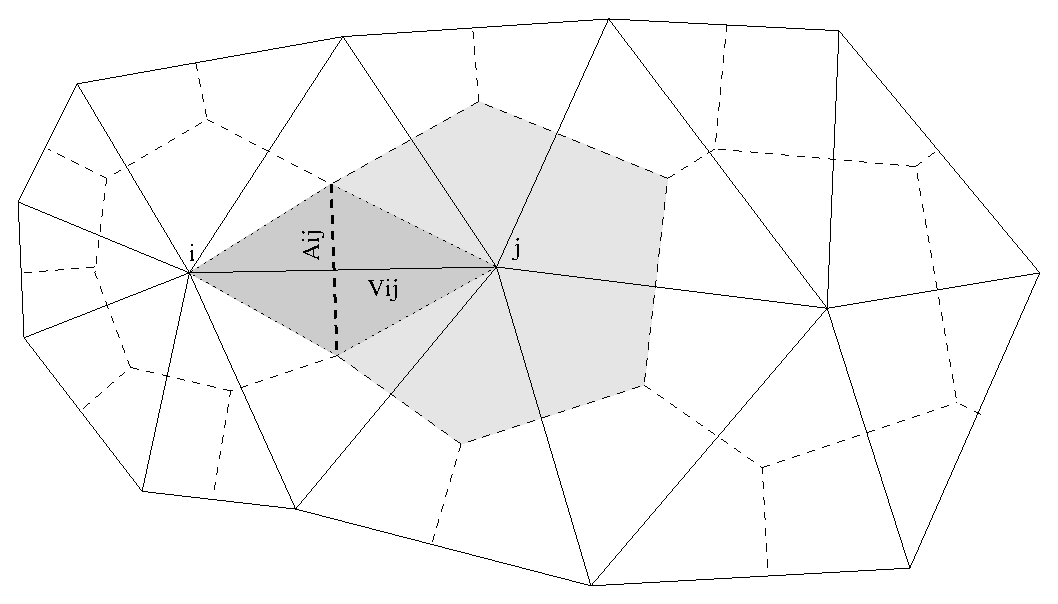
\includegraphics[width=0.9\textwidth]{figures/voronoi.eps}
 \caption{Schematic of a Delaunay mesh with its dual Voronoi diagram, where the box containing vertex $j$ is highlighted.
    The function \lstinline|voronoi()| computes and stores the Voronoi volume $V_{[i,j]}$ and the interface area $A_{[i,j]}$ associated with each edge $[i,j]$.
    The total box volume associated with each vertex is also stored on the vertex.}
 \label{fig:voronoi}
\end{figure}

 \subsection{Voronoi Information}
 A Voronoi diagram of a Delaunay tessellation (or triangulation) is a decomposition of the mesh into certain boxes containing one vertex each.
 The boxes have the property that all points inside the box are closer to the vertex within the box than to any other vertex in the mesh.
 By simple geometric arguments one finds that the corners of Voronoi boxes are given by the circumcenters of the triangles.

 The function \lstinline|apply_voronoi()| computes the volumes and interfaces associated with a Voronoi diagram. The following values are stored on the mesh (cf.~Fig.~\ref{fig:voronoi})
 \begin{itemize}
  \item The volume $V_{[i,j]}$ of the polyhedron centered around the edge $[i,j]$ with edges given by the connections of the vertices $i$ and $j$ with the circumcenters of the coboundary cells of the edge is stored on the edge $[i,j]$.
  \item The interface area $A_{[i,j]}$ of the boxes for the vertices $i$ and $j$ on the edge $[i,j]$.
  \item The box volume $V_i$ of the box containing vertex $i$ for each vertex $i$.
 \end{itemize}
 The voronoi values are stored in the corresponding accessors/containers using the lines
 \begin{lstlisting}
  using namespace viennagrid;
  typedef result_of::voronoi_cell_contribution<ConstCellHandleType>::type ContributionType;

  // define containers for interface contributions and accessors
  std::vector<double>           interface_areas;
  std::vector<ContributionType> interface_contrib;

  result_of::accessor< std::vector<double>, EdgeType >::type           interface_areas_accessor(interface_areas);
  result_of::accessor< std::vector<ContributionType>, EdgeType >::type interfaces_contrib_accessor(interface_contrib);

  // define containers for box volumes and accessors on vertices
  std::vector<double>           vertex_box_volumes;
  std::vector<ContributionType> vertex_box_volume_contrib;

  result_of::accessor< std::vector<double>, VertexType >::type           vertex_box_volumes_accessor(vertex_box_volumes);
  result_of::accessor< std::vector<ContributionType>, VertexType >::type vertex_box_volume_contrib_accessor(vertex_box_volume_contrib);

  // define containers for box volumes and accessors on edges
  std::vector<double>           edge_box_volumes;
  std::vector<ContributionType> edge_box_volume_contrib;

  result_of::accessor< std::vector<double>, EdgeType >::type           edge_box_volumes_accessor(edge_box_volumes);
  result_of::accessor< std::vector<ContributionType>, EdgeType >::type edge_box_volume_contrib_accessor(edge_box_volume_contrib);

  apply_voronoi<CellType>(
        mesh,
        interface_areas_accessor,    interfaces_contrib_accessor,
        vertex_box_volumes_accessor, vertex_box_volume_contrib_accessor,
        edge_box_volumes_accessor,   edge_box_volume_contrib_accessor)
  );
 \end{lstlisting}
 Note that the interface for \lstinline|apply_voronoi()| is purely defined via the abstract accessors defined in Chapter \ref{chap:data}.
 Thus, the user is free to pick any container as long as a suitable wrapper fulfilling the accessor concept is provided.
 
